\chapter{A Complete MSCKF in the Plane}
\label{ch:planar}

\begin{objectives}
\begin{itemize}
  \item Build a complete MSCKF for a robot moving in a plane, small enough that every Jacobian can be derived by hand in a few lines.
  \item Meet every ingredient of the full filter in its simplest form: nominal and error state, propagation, cloning, triangulation,
        nullspace projection, gating, update and marginalization.
  \item See, in a three-view example, what the projected residual actually measures.
  \item Run the filter in simulation and check its accuracy and consistency.
  \item Identify the unobservable directions, and list exactly what changes in three dimensions.
\end{itemize}
\end{objectives}

The previous three chapters described the MSCKF in full generality. This chapter does something different: it builds the whole
filter for a toy problem in which nothing is hidden. A robot drives on a plane, measures its speed and turn rate, and carries a
camera that sees the world as a line of pixels. Every equation is derived, every Jacobian is checked against geometric
intuition, and the result is run in a simulation whose code accompanies these notes
(\code{scripts/planar\_sims.py}, about two hundred lines of Python). If the general chapters felt abstract, work through this one with a
pencil; afterwards, the three-dimensional filter differs only in details that \cref{sec:planar-to-3d} lists one by one.

\begin{projectlink}[what this chapter does and does not give away]
The planar Jacobians below are derived in full because the planar system is not the project's system. The three-dimensional Jacobians
($F_c$, $G_c$, the pose and camera $H$, the cloning $J$) differ precisely where the difficulty lies: rotations that do not commute, the frozen local
perturbation, gravity, biases, and the reset Jacobian. Deriving them remains your task (AGENTS.md Guardrail 4). Use this chapter as the
template: the same procedure (perturb, expand to first order, read off the coefficient), and the same finite-difference checks.
\end{projectlink}

% ------------------------------------------------------------------------------
\section{The planar world}
\label{sec:planar-world}
\index{MSCKF!planar}\index{planar MSCKF}

\subsection{Frames and pose}

The world frame $W$ is a fixed plane with axes $x_w, y_w$. The robot carries a body frame $B$ with $x_b$ pointing forward and
$y_b$ to the left. Its pose is the position $p \in \R^2$ of the body origin in $W$ and the heading $\psi$, the angle from $x_w$ to $x_b$. The
rotation
\begin{equation}
  R(\psi) = \begin{bmatrix} \cos\psi & -\sin\psi \\ \sin\psi & \cos\psi \end{bmatrix}
\end{equation}
maps body-frame vectors to the world frame, $v_w = R(\psi)\,v_b$: it plays the role of $R_{wb}$ (AGENTS.md C1). A point $p_f$ given in $W$ has
body coordinates $p_b = R(\psi)\T(p_f - p)$.

\subsection{The planar skew matrix}

The matrix\index{planar skew matrix}
\begin{equation}
  \Omega = \begin{bmatrix} 0 & -1 \\ 1 & 0 \end{bmatrix}
\end{equation}
rotates a vector by $+90^\circ$: $\Omega\,(a_1, a_2) = (-a_2, a_1)$. It is the planar version of the skew matrix: for a rotation about the
$z$-axis, $\sx{\omega e_z}$ acts on the $xy$-plane exactly as $\omega\,\Omega$ (compare \cref{sec:so2}).

\begin{lemma}[Properties of $\Omega$]
\label{lem:omega}
For all $\psi$, $\delta$ and $a \in \R^2$:
\begin{enumerate}
  \item $\Omega\T = -\Omega$, $\Omega^2 = -I$, and $a\T\Omega a = 0$;
  \item $R(\psi) = \cos\psi\,I + \sin\psi\,\Omega = \exp(\psi\,\Omega)$;
  \item $R(\psi)\,\Omega = \Omega\,R(\psi)$ and $R(\psi)\T\Omega = \Omega R(\psi)\T$;
  \item $\dfrac{\dd}{\dd\psi}R(\psi) = \Omega R(\psi)$, and $R(\psi + \delta) = R(\psi)\big(I + \delta\,\Omega\big) + O(\delta^2)$;
  \item $R(\psi + \delta)\T = (I - \delta\,\Omega)\,R(\psi)\T + O(\delta^2)$.
\end{enumerate}
\end{lemma}
\begin{proof}
(1) Direct multiplication; $a\T\Omega a = -a_1a_2 + a_2a_1 = 0$. (2) Read off the entries of $\cos\psi\,I + \sin\psi\,\Omega$. For the exponential,
$\Omega^2 = -I$ gives $\Omega^{2k} = (-1)^kI$ and $\Omega^{2k+1} = (-1)^k\Omega$, so the series splits into the cosine and sine series. (3) By (2),
$R(\psi)$ is a combination of $I$ and $\Omega$, and both commute with $\Omega$; transpose for the second identity. (4) Differentiate (2):
$-\sin\psi\,I + \cos\psi\,\Omega = \Omega(\cos\psi\,I + \sin\psi\,\Omega)$, using $\Omega^2 = -I$. Then $R(\psi + \delta) = R(\psi)R(\delta)$ and
$R(\delta) = I + \delta\,\Omega + O(\delta^2)$ by (2). (5) Transpose (4) and use $\Omega\T = -\Omega$.
\end{proof}

Property (3) is the reason the plane is easy: rotations commute with each other and with $\Omega$, so $R(\hat\psi)R(\delta) = R(\delta)R(\hat\psi)$
and a heading error can be added on either side. In three dimensions neither is true, and the frozen local perturbation of AGENTS.md C4 is a
real choice with real consequences.

% ------------------------------------------------------------------------------
\section{Sensors}

\subsection{Odometry}

Wheel odometry plays the part of the IMU. It measures the forward speed $v$ and the turn rate $\omega$ in the body frame, with white noise:
\begin{equation}
  v_m = v + n_v, \qquad \omega_m = \omega + n_\omega, \qquad
  \E[n_v(t)n_v(s)] = \sigma_v^2\,\delta(t - s),\quad \E[n_\omega(t)n_\omega(s)] = \sigma_\omega^2\,\delta(t - s).
  \label{eq:planar-odometry}
\end{equation}
As for the IMU (\cref{sec:ct-noise}), $\sigma_v$ and $\sigma_\omega$ are continuous-time noise densities, in $\mathrm{m/s/\sqrt{Hz}}$ and
$\mathrm{rad/s/\sqrt{Hz}}$; a sample at period $\Dt$ has standard deviation $\sigma/\sqrt{\Dt}$. The robot does not slip sideways, so the
kinematics are
\begin{equation}
  \dot p = R(\psi)\,e_1\,v, \qquad \dot\psi = \omega, \qquad e_1 = (1, 0).
  \label{eq:planar-kinematics}
\end{equation}
There are no biases and no gravity. Both appear in the exercises.

\subsection{A one-dimensional camera}

The camera sits at the body origin and looks along $x_b$. A planar pinhole camera has a one-dimensional image: the point
$p_b = (x, y)$ in front of the camera ($x > 0$) is projected onto the \emph{image line} $x = 1$ at the normalized coordinate
\begin{equation}
  z = \pi(p_b) + n_z = \frac{y}{x} + n_z, \qquad n_z \sim \N(0, \sigma_z^2).
  \label{eq:planar-camera}
\end{equation}
This is the planar analog of the normalized image coordinates of \cref{ch:camera}: a real 1D sensor with focal length $f$ (in pixels) and
principal point $c$ would report $u = fz + c$, so a pixel noise $\sigma_{px}$ corresponds to $\sigma_z = \sigma_{px}/f$. The camera measures only the
\emph{bearing}\index{bearing} $\beta = \arctan z$ of the point; its range is invisible, exactly as depth is invisible to a monocular camera in space.

\begin{figure}[t]
\centering
\begin{tikzpicture}[scale=1.3, >=stealth]
  % world frame
  \draw[->, black!60] (0,0) -- (0.9,0) node[right, font=\footnotesize] {$x_w$};
  \draw[->, black!60] (0,0) -- (0,0.9) node[above, font=\footnotesize] {$y_w$};
  \node[below left, font=\footnotesize, black!60] at (0,0) {$W$};
  % robot position and heading
  \coordinate (B) at (2.2,0.5);
  \draw[->, black!70] (0,0) -- (B) node[pos=0.5, above left=-1pt, font=\footnotesize] {$p$};
  \draw[dashed, black!40] (B) -- ++(1.3,0);
  \draw[->, black!70] ($(B)+(1.0,0)$) arc (0:25:1.0) node[pos=0.5, right, font=\footnotesize] {$\psi$};
  \begin{scope}[shift={(B)}, rotate=25]
    % body axes
    \draw[->, thick, primary] (0,0) -- (1.55,0) node[pos=1, above=1pt, font=\footnotesize] {$x_b$};
    \draw[->, thick, primary] (0,0) -- (0,1.0) node[above, font=\footnotesize] {$y_b$};
    \fill[primary] (0,0) circle (1.6pt);
    % image line x_b = 1
    \draw[very thick, plotorange] (1,-0.3) -- (1,1.25) node[above, font=\footnotesize] {image line $x_b = 1$};
    % feature and its ray
    \coordinate (F) at (3.6,1.5);
    \draw[dashed, plotgreen!60!black] (0,0) -- (F);
    \fill[plotgreen!70!black] (F) circle (2pt) node[right=2pt, font=\footnotesize] {$p_f$};
    % image point
    \fill[plotorange] (1,{1.5/3.6}) circle (1.6pt);
    \node[font=\footnotesize, plotorange!80!black, anchor=east] at (0.97,{1.5/3.6 + 0.1}) {$z$};
    % bearing angle
    \draw[black!60] (0.6,0) arc (0:22.6:0.6);
    \node[font=\scriptsize, black!70] at (0.78,0.14) {$\beta$};
    % depth and lateral offset of the feature
    \draw[|<->|, black!50] (0,-0.55) -- (3.6,-0.55) node[pos=1, right=2pt, font=\scriptsize, black!70] {$x$ (depth, not observed)};
    \draw[dotted, black!40] (3.6,-0.55) -- (3.6,1.5);
    \node[font=\scriptsize, black!70, anchor=west] at (3.62,0.6) {$y$};
  \end{scope}
\end{tikzpicture}
\caption{The planar robot and its one-dimensional camera. The feature $p_f$ has body coordinates $(x, y)$; the camera reports where the ray to it
crosses the image line $x_b = 1$, the normalized coordinate $z = y/x = \tan\beta$. Moving the feature along the ray does not change $z$.}
\label{fig:planar-setup}
\end{figure}

% ------------------------------------------------------------------------------
\section{State, error state and propagation}

\subsection{The state}

The filter state is the current robot pose followed by $N$ clones of past poses, taken at image times:
\begin{equation}
  x = \big(p,\ \psi,\ \ p_1, \psi_1,\ \dots,\ p_N, \psi_N\big) \in \R^{3 + 3N}.
\end{equation}
Because planar rotations commute, the retraction is ordinary addition (wrapping angles to $(-\pi, \pi]$): $p = \hat p + \delta p$ and
$\psi = \hat\psi + \delta\psi$, which is simultaneously the local and the global perturbation, and
$\delta x = (\delta p, \delta\psi, \delta p_1, \delta\psi_1, \dots)$. The state has no velocity block, since speed is measured directly rather than
integrated from accelerations.

\subsection{Nominal propagation}

Between odometry samples the inputs are held constant. The nominal state is integrated with the midpoint rule for the heading,
\begin{equation}
  \hat p_{k+1} = \hat p_k + R\big(\hat\psi_k + \tfrac12\omega_m\Dt\big)\,e_1\,v_m\Dt, \qquad \hat\psi_{k+1} = \hat\psi_k + \omega_m\Dt,
  \label{eq:planar-nominal}
\end{equation}
which is the exact solution for an arc travelled at constant speed and turn rate, up to the factor $\sin(\omega\Dt/2)/(\omega\Dt/2) = 1 - O(\Dt^2)$
on its length. Clones do not move.

\subsection{Error dynamics}

\begin{proposition}[Planar error dynamics]
\label{prop:planar-error}
To first order in the errors and the noise, the robot error obeys $\dot{\delta x}_R = F_c\,\delta x_R + G_c\,n$ with
$\delta x_R = (\delta p, \delta\psi)$, $n = (n_v, n_\omega)$ and
\begin{equation}
  F_c = \begin{bmatrix} 0_{2\times2} & \Omega\,R(\hat\psi)\,e_1\,v_m \\ 0_{1\times2} & 0 \end{bmatrix}, \qquad
  G_c = \begin{bmatrix} -R(\hat\psi)\,e_1 & 0_{2\times1} \\ 0 & -1 \end{bmatrix}.
  \label{eq:planar-FG}
\end{equation}
The top-right block equals $\Omega\,\dot{\hat p}$: a heading error $\delta\psi$ makes the position error grow perpendicular to the direction of travel.
\end{proposition}
\begin{proof}
Write the true quantities as nominal plus error, $\psi = \hat\psi + \delta\psi$, and the true inputs as measured minus noise,
$v = v_m - n_v$, $\omega = \omega_m - n_\omega$. For the heading, $\dot{\delta\psi} = \dot\psi - \dot{\hat\psi} = (\omega_m - n_\omega) - \omega_m = -n_\omega$.
For the position, by \cref{lem:omega}(4),
\begin{align*}
  \dot p &= R(\hat\psi + \delta\psi)\,e_1\,(v_m - n_v) = R(\hat\psi)(I + \delta\psi\,\Omega)\,e_1\,(v_m - n_v) + O(\delta\psi^2) \\
  &= R(\hat\psi)e_1v_m + \delta\psi\,R(\hat\psi)\Omega e_1\,v_m - R(\hat\psi)e_1\,n_v + \dots,
\end{align*}
dropping the product $\delta\psi\,n_v$. Subtracting $\dot{\hat p} = R(\hat\psi)e_1v_m$ and using $R\Omega = \Omega R$ gives
$\dot{\delta p} = \Omega R(\hat\psi)e_1v_m\,\delta\psi - R(\hat\psi)e_1\,n_v$, which is the first block row.
\end{proof}

Discretization follows \cref{ch:linsys} exactly: $\Phi \approx I + F_c\Dt$, and $Q_d \approx G_c Q_c G_c\T\Dt$ with $Q_c = \mathrm{diag}(\sigma_v^2, \sigma_\omega^2)$.
The covariance is propagated block by block, with static clones:
\begin{equation}
  P_{RR} \gets \Phi P_{RR}\Phi\T + Q_d, \qquad P_{RC} \gets \Phi P_{RC}, \qquad P_{CC} \text{ unchanged},
\end{equation}
followed by symmetrization.

For the observability analysis we also need the transition matrix of the discrete integrator \eqref{eq:planar-nominal} itself, without the
$O(\Dt^2)$ truncation of $I + F_c\Dt$.

\begin{proposition}[Exact discrete error transition]
\label{prop:planar-phi}
Linearizing \eqref{eq:planar-nominal} in the errors gives $\delta p_{k+1} = \delta p_k + \Omega\,(\hat p_{k+1} - \hat p_k)\,\delta\psi_k + (\text{noise})$ and
$\delta\psi_{k+1} = \delta\psi_k + (\text{noise})$, that is
\begin{equation}
  \Phi_k = \begin{bmatrix} I_2 & \Omega\,(\hat p_{k+1} - \hat p_k) \\ 0 & 1 \end{bmatrix}.
  \label{eq:planar-phi}
\end{equation}
\end{proposition}
\begin{proof}
The true state obeys the same recursion with the true heading and inputs. A heading error $\delta\psi_k$ rotates the step
$s = R(\hat\psi_k + \tfrac12\omega_m\Dt)e_1v_m\Dt$ into $R(\delta\psi_k)s \approx s + \delta\psi_k\,\Omega s$, and $s = \hat p_{k+1} - \hat p_k$.
\end{proof}

The transition depends on the estimates only through the displacement $\hat p_{k+1} - \hat p_k$. Over many steps the products of such matrices
telescope, $\Phi_{k-1}\cdots\Phi_0 = \begin{bmatrix} I & \Omega(\hat p_k - \hat p_0) \\ 0 & 1\end{bmatrix}$, provided each displacement is computed from
\emph{the same} estimates; \cref{ch:observability} shows what happens when it is not.

% ------------------------------------------------------------------------------
\section{Cloning and marginalization}

At an image time the robot pose is copied into a new clone. The clone is an exact copy, so its error is the robot's error:
$\delta p_{N+1} = \delta p$, $\delta\psi_{N+1} = \delta\psi$. With the robot block first, \cref{prop:augmentation} gives
\begin{equation}
  P \gets JPJ\T, \qquad J = \begin{bmatrix} I_{3+3N} \\ \begin{bmatrix} I_3 & 0_{3\times3N} \end{bmatrix} \end{bmatrix}.
\end{equation}
No linearization is involved: the copy is exact, which is why the new clone's covariance block and its cross-covariances equal the robot's
\emph{exactly}. When the window is full, the features that the oldest clone observed are processed first, then the clone is marginalized by
deleting its three rows and columns, as in \cref{ch:cloning}.

% ------------------------------------------------------------------------------
\section{The feature measurement}

\subsection{Residual and Jacobians}

Feature $j$, at the unknown position $p_f$, is observed by clone $i$ at the coordinate $z_i$. With the triangulated estimate $\hat p_f$ and
the clone estimate $(\hat p_i, \hat\psi_i)$, the predicted body-frame point and the residual are
\begin{equation}
  \hat p_{b,i} = R(\hat\psi_i)\T(\hat p_f - \hat p_i) = (\hat x_i, \hat y_i), \qquad r_i = z_i - \hat y_i/\hat x_i .
\end{equation}

\begin{proposition}[Planar camera Jacobians]
\label{prop:planar-H}
Let $\hat z_i = \hat y_i/\hat x_i$ and $J_\pi = \frac{1}{\hat x_i}\begin{bmatrix} -\hat z_i & 1\end{bmatrix}$, the derivative of $y/x$ with respect to $(x, y)$.
To first order, $r_i \approx H_{x,i}\,\delta x + H_{f,i}\,\delta p_f + n_{z,i}$, where $H_{x,i}$ is zero except in the three columns of clone $i$, and
\begin{equation}
  \frac{\partial r_i}{\partial\delta p_i} = -J_\pi R(\hat\psi_i)\T, \qquad
  \frac{\partial r_i}{\partial\delta\psi_i} = -J_\pi\Omega\,\hat p_{b,i} = -\big(1 + \hat z_i^2\big), \qquad
  H_{f,i} = \frac{\partial r_i}{\partial\delta p_f} = J_\pi R(\hat\psi_i)\T .
  \label{eq:planar-H}
\end{equation}
\end{proposition}
\begin{proof}
The measurement is $z_i = \pi(p_{b,i}) + n_{z,i}$ with $p_{b,i} = R(\psi_i)\T(p_f - p_i)$, so $r_i = z_i - \pi(\hat p_{b,i}) \approx J_\pi\,(p_{b,i} - \hat p_{b,i}) + n_{z,i}$:
we need the first-order change of $p_{b,i}$. Substituting $p_i = \hat p_i + \delta p_i$, $p_f = \hat p_f + \delta p_f$ and, by \cref{lem:omega}(5),
$R(\hat\psi_i + \delta\psi_i)\T \approx (I - \delta\psi_i\Omega)R(\hat\psi_i)\T$,
\begin{equation*}
  p_{b,i} \approx (I - \delta\psi_i\Omega)\,R(\hat\psi_i)\T(\hat p_f - \hat p_i + \delta p_f - \delta p_i)
  \approx \hat p_{b,i} - \delta\psi_i\,\Omega\,\hat p_{b,i} + R(\hat\psi_i)\T(\delta p_f - \delta p_i).
\end{equation*}
Multiplying by $J_\pi$ gives the three Jacobians. For the heading term,
$J_\pi\Omega\hat p_{b,i} = \frac{1}{\hat x}\begin{bmatrix} -\hat z & 1\end{bmatrix}\begin{bmatrix} -\hat y \\ \hat x\end{bmatrix} = \frac{\hat z\hat y + \hat x}{\hat x} = \hat z^2 + 1$,
using $\hat y = \hat z\hat x$.
\end{proof}

Each block has a clear meaning.
\begin{itemize}
  \item \textbf{Rotation} shifts every bearing by the same angle: turning the robot left by $\delta\psi$ decreases every bearing by $\delta\psi$, and since
        $z = \tan\beta$, $\dd z = (1 + z^2)\,\dd\beta$. The heading column does not depend on the depth at all. This is why a camera measures
        rotation so well, even from points at infinity.
  \item \textbf{Translation} enters through $J_\pi$, which carries the factor $1/\hat x$: moving the robot shifts near points a lot and far points
        hardly at all. This is \emph{parallax}\index{parallax}, the only way a camera senses translation.
  \item \textbf{The feature} enters with the opposite sign of the clone position: moving the feature by $\delta p_f$ looks, to this camera, exactly like
        moving the robot by $-\delta p_f$. Only the relative position $p_f - p_i$ matters.
\end{itemize}

\begin{implnote}[check the Jacobians numerically anyway]
Even a three-line derivation deserves a finite-difference check (\cref{sec:numdiff}). Perturb each clone coordinate and the feature by
$\varepsilon = 10^{-6}$, recompute $\pi(R(\psi_i)\T(p_f - p_i))$, and compare the difference quotients with \eqref{eq:planar-H}; agreement to
about $10^{-8}$ is expected. Flip the sign of the heading term and the check fails at once, which is the point.
\end{implnote}

\subsection{Triangulation}
\index{triangulation!planar}

To linearize we need $\hat p_f$. Observation $i$ says that $p_f$ lies on the ray from $\hat p_i$ in the direction $d_i = R(\hat\psi_i)\,(1, z_i)$,
that is $p_f - \hat p_i = \lambda_i d_i$ for some depth $\lambda_i > 0$. The depth is eliminated with the normal $n_i = \Omega d_i$, which is perpendicular to the ray
(\cref{lem:omega}(1)):
\begin{equation}
  n_i\T(p_f - \hat p_i) = 0, \qquad i = 1, \dots, M \qquad\Longrightarrow\qquad
  \underbrace{\begin{bmatrix} n_1\T \\ \vdots \\ n_M\T\end{bmatrix}}_{A}\,p_f = \underbrace{\begin{bmatrix} n_1\T\hat p_1 \\ \vdots \\ n_M\T\hat p_M\end{bmatrix}}_{b}.
  \label{eq:planar-tri}
\end{equation}
Two non-parallel rays determine $p_f$, and more rays give an overdetermined system solved by least squares (\cref{sec:least-squares}).
If the rays are nearly parallel (too little parallax), $A$ is ill-conditioned and the feature is rejected; the simulation rejects
features with $\kappa(A) > 10^4$. The linear solution minimizes algebraic distances, not the measurement errors, so it is refined by a few
Gauss--Newton iterations (\cref{sec:gauss-newton}) on $\sum_i (z_i - \pi(R(\hat\psi_i)\T(p_f - \hat p_i)))^2$, whose Jacobian rows are exactly the
$H_{f,i}$ of \eqref{eq:planar-H}. Finally every depth $\hat x_i$ must be positive (in the simulation, at least \SI{0.2}{m}): a point behind a
camera is a failed triangulation, not a measurement.

% ------------------------------------------------------------------------------
\section{Eliminating the feature}

Stacking the $M$ observations of feature $j$ gives $r_j \approx H_{x,j}\,\delta x + H_{f,j}\,\delta p_f + n_j$ with $H_{f,j} \in \R^{M\times2}$. If the
rays are not parallel, $H_{f,j}$ has rank 2 and its left nullspace has dimension $M - 2$: \emph{a feature seen $M$ times gives $M - 2$ constraints on
the poses}. Two observations give none, because two rays in a plane always intersect, so any pair of bearings is consistent with some
feature position. With $A_j$ an orthonormal basis of the left nullspace (computed by QR, \cref{prop:qr-nullspace}),
\begin{equation}
  r_{o,j} = A_j\T r_j \approx A_j\T H_{x,j}\,\delta x + A_j\T n_j, \qquad \Cov(A_j\T n_j) = \sigma_z^2 I_{M-2},
\end{equation}
exactly as in \cref{ch:msckfupdate}. For three observations the nullspace is a single vector, and in $\R^3$ there is a closed form for it.

\begin{proposition}[Three views]
\label{prop:three-views}
If $M = 3$ and the columns $h_1, h_2 \in \R^3$ of $H_{f,j}$ are linearly independent, the left nullspace of $H_{f,j}$ is spanned by the cross product
$a = h_1\times h_2$.
\end{proposition}
\begin{proof}
$a\T h_1 = (h_1\times h_2)\cdot h_1 = 0$ and likewise for $h_2$ (\cref{sec:skew}), and $a \ne 0$ because the columns are independent. The
nullspace has dimension $3 - 2 = 1$, so $a$ spans it.
\end{proof}

\begin{worked}[what three views measure]
Let the robot face along $x_w$ ($\hat\psi_i = 0$) at the three positions $\hat p_1 = (0, -1)$, $\hat p_2 = (0, 0)$, $\hat p_3 = (0, 1)$, a sideways motion with two
equal baselines, and let the feature be at $\hat p_f = (4, 0)$. The body-frame points are $(4, 1)$, $(4, 0)$ and $(4, -1)$, so
$\hat z = (\tfrac14, 0, -\tfrac14)$ and, by \eqref{eq:planar-H},
\begin{equation*}
  H_f = \begin{bmatrix} -\tfrac{1}{16} & \tfrac14 \\ 0 & \tfrac14 \\ \tfrac{1}{16} & \tfrac14 \end{bmatrix}, \qquad
  h_1\times h_2 = \tfrac{1}{64}(-1, 2, -1), \qquad a = \tfrac{1}{\sqrt6}(1, -2, 1).
\end{equation*}
The projected residual is $r_o = (r_1 - 2r_2 + r_3)/\sqrt6$, a \emph{second difference}. The reason is visible in the geometry: for cameras translating
sideways at a fixed heading, $z_i = (y_f - y_i)/x_f$ is a linear function of the camera position $y_i$, whatever the feature. A feature can absorb
any offset and any slope of the three residuals; only their curvature is left for the poses to explain.

The projected Jacobian is $H_o = a\T H_x$, with clone blocks $(\delta p_x, \delta p_y, \delta\psi)$
\begin{equation*}
  H_o = \tfrac{1}{\sqrt6}\Big[\ \big(\tfrac{1}{16}, -\tfrac14, -\tfrac{17}{16}\big)\ \ \big(0, \tfrac12, 2\big)\ \ \big(-\tfrac{1}{16}, -\tfrac14, -\tfrac{17}{16}\big)\ \Big],
\end{equation*}
since the clone blocks of $H_x$ are $\big(\tfrac{1}{16}, -\tfrac14, -\tfrac{17}{16}\big)$, $\big(0, -\tfrac14, -1\big)$ and $\big(-\tfrac{1}{16}, -\tfrac14, -\tfrac{17}{16}\big)$.
Now test what it can see by multiplying $H_o$ by a pose perturbation:
\begin{itemize}
  \item \emph{Translate all three clones} by the same $(\delta_x, \delta_y)$: $H_o\,\delta x = \tfrac{1}{\sqrt6}\big[\tfrac{1}{16} - \tfrac{1}{16}\big]\delta_x + \tfrac{1}{\sqrt6}\big[-\tfrac14 + \tfrac12 - \tfrac14\big]\delta_y = 0$. Invisible.
  \item \emph{Rotate everything} about the origin by $\delta$: each clone moves by $\delta\,\Omega\hat p_i$, that is $(\delta, 0)$, $(0, 0)$, $(-\delta, 0)$, and turns by $\delta$.
        The result is $\tfrac{\delta}{\sqrt6}\big[\tfrac{1}{16} - \tfrac{17}{16} + 2 + \tfrac{1}{16} - \tfrac{17}{16}\big] = 0$. Invisible.
  \item \emph{Scale} the configuration about the origin: $\delta p_1 = (0, -s)$, $\delta p_3 = (0, s)$, $\delta p_2 = 0$, giving $\tfrac{s}{\sqrt6}\big[\tfrac14 - \tfrac14\big] = 0$. Invisible:
        a camera cannot measure scale.
  \item \emph{Move only the middle clone} sideways by $\delta_y$: $H_o\,\delta x = \delta_y/(2\sqrt6) \ne 0$. Visible: the camera measures the \emph{ratio} of the two baselines.
  \item \emph{Turn only the middle clone} by $\delta$: $H_o\,\delta x = 2\delta/\sqrt6 \ne 0$. Visible: relative headings are measured directly.
\end{itemize}
This small example contains the whole story of monocular visual odometry: relative rotations and the shape of the trajectory are observed, while
the global position, the global heading and the scale are not. In the filter, the odometry speed supplies the scale, and nothing supplies the
global pose.
\end{worked}

\paragraph{Gating, stacking and the update.} Each projected residual is gated with $\gamma_j = r_{o,j}\T(H_{o,j}PH_{o,j}\T + \sigma_z^2I)\inv r_{o,j}
< \chi^2_{0.95}(M - 2)$, the survivors are stacked into one measurement, and the update is the generic one of \cref{ch:updates}: $S = HPH\T + \sigma_z^2I$, the
gain by a linear solve, the Joseph form, symmetrization. Injection adds the correction to the robot and to every clone,
$\hat p_i \gets \hat p_i + \delta\hat p_i$, $\hat\psi_i \gets \hat\psi_i + \delta\hat\psi_i$ (wrapped). There is no reset Jacobian: after injection the new error is
$\psi - (\hat\psi + \delta\hat\psi) = \delta\psi - \delta\hat\psi$, whose derivative with respect to $\delta\psi$ is exactly 1. In three dimensions the corresponding
derivative is $I - \tfrac12\sx{\delta\hat\theta}$ (\cref{sec:reset}), because rotations do not commute.

% ------------------------------------------------------------------------------
\section{The complete filter}

\Cref{alg:planar-msckf} collects the steps; it is the full MSCKF of \cref{ch:fullalgo} with the planar models substituted.

\begin{algorithm}[t]
\caption{Planar MSCKF}
\label{alg:planar-msckf}
\begin{algorithmic}[1]
\Require initial pose estimate and covariance, window size $N_{\max}$
\For{each odometry sample $(v_m, \omega_m)$ with period $\Dt$}
  \State propagate $P$ with $\Phi = I + F_c\Dt$, $Q_d = G_cQ_cG_c\T\Dt$ (\cref{prop:planar-error}); clones static
  \State propagate the nominal pose with \eqref{eq:planar-nominal}
  \If{an image arrives at this time}
    \State collect tracks that ended (feature not seen in this image)
    \If{$N = N_{\max}$} also collect tracks whose first observation is the oldest clone \EndIf
    \For{each collected track with $M \ge 3$}
      \State triangulate \eqref{eq:planar-tri} + Gauss--Newton; reject on parallax or negative depth
      \State build $r_j, H_{x,j}, H_{f,j}$ with \eqref{eq:planar-H}; project onto the left nullspace of $H_{f,j}$
      \State gate with $\chi^2_{0.95}(M - 2)$; keep or count the rejection
    \EndFor
    \State stack the survivors; EKF update (Joseph); inject into the robot and all clones
    \If{$N = N_{\max}$} marginalize the oldest clone \EndIf
    \State clone the current pose; append this image's observations to their tracks
  \EndIf
\EndFor
\end{algorithmic}
\end{algorithm}

The heart of the filter, the per-feature residual, is short enough to show in full. It mirrors \eqref{eq:planar-H} line by line;
\code{OM} is $\Omega$ and \code{rot(psi)} is $R(\psi)$.

\begin{lstlisting}[style=py]
def feature_residual(self, obs):              # obs: list of (clone id, z)
    pf = self.triangulate(obs)                # linear + Gauss-Newton, with checks
    if pf is None:
        return None
    m = len(obs)
    Hx, Hf, r = np.zeros((m, self.n)), np.zeros((m, 2)), np.zeros(m)
    for row, (cid, z) in enumerate(obs):
        k = self.clone_index(cid)
        _, p_i, psi_i = self.clones[k]
        Rt = rot(psi_i).T
        pb = Rt @ (pf - p_i)                  # feature in the body frame of the clone
        Jpi = np.array([-pb[1] / pb[0]**2, 1.0 / pb[0]])   # d(y/x)/d(x, y)
        col = 3 + 3 * k                       # columns of clone k
        Hx[row, col:col + 2] = -Jpi @ Rt      # clone position
        Hx[row, col + 2] = -Jpi @ (OM @ pb)   # clone heading: -(1 + z^2)
        Hf[row] = Jpi @ Rt                    # feature position
        r[row] = z - pb[1] / pb[0]
    Q, _ = qr(Hf, mode="full")
    A = Q[:, 2:]                              # orthonormal basis of the left nullspace
    Ho, ro = A.T @ Hx, A.T @ r
    S = Ho @ self.P @ Ho.T + self.sig_z**2 * np.eye(m - 2)
    if ro @ np.linalg.solve(S, ro) > chi2.ppf(0.95, m - 2):
        self.rejected += 1                    # gated out: counted, never silent
        return None
    return Ho, ro
\end{lstlisting}

A production implementation would not form \code{A}; it would apply the Householder reflections of \cref{alg:nullspace-householder} to
$[H_f\ |\ H_x\ |\ r]$, and it would work only with the non-zero clone columns of $H_x$.

% ------------------------------------------------------------------------------
\section{Simulation results}

\begin{table}[t]
\centering
\small
\caption{Planar simulation parameters.}
\label{tab:planar-sim}
\begin{tabular}{@{}ll@{}}
\toprule
Trajectory & circle of radius \SI{10}{m} at \SI{1}{m/s} and \SI{0.1}{rad/s}, \SI{90}{s} (1.4 laps) \\
Odometry & \SI{100}{Hz}; $\sigma_v = 0.01~\mathrm{m/s/\sqrt{Hz}}$, $\sigma_\omega = 0.02~\mathrm{rad/s/\sqrt{Hz}}$ \\
Camera & \SI{10}{Hz}; field of view $\pm50^\circ$; depths \SIrange{1}{15}{m}; $\sigma_z = 0.003$ (\SI{1.5}{px} at $f = \SI{500}{px}$) \\
Landmarks & 260, in two rings (radii \SIrange{3}{7}{m} and \SIrange{13}{19}{m}) \\
Window & $N_{\max} = 10$ clones (\SI{1}{s}) \\
Initial uncertainty & $\sigma_p = \SI{1}{cm}$ per axis, $\sigma_\psi = \SI{3}{mrad}$ \\
\bottomrule
\end{tabular}
\end{table}

\Cref{tab:planar-sim} lists the simulation set-up. The truth moves exactly on the circle; odometry samples are drawn with the noise densities
of the table, and each landmark inside the field of view and depth range produces a bearing with noise $\sigma_z$. Dead reckoning, the same nominal
integration without any camera update, serves as the baseline.

\begin{figure}[t]
\centering
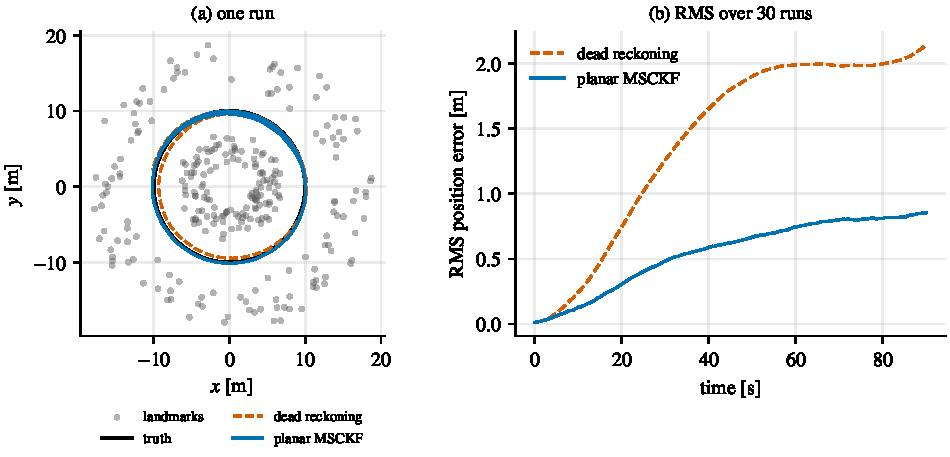
\includegraphics[width=\linewidth]{fig_planar_traj.pdf}
\caption{Planar MSCKF versus dead reckoning. (a) One run. (b) Root-mean-square position error over 30 Monte Carlo runs: after
\SI{90}{s}, \SI{0.85}{m} for the MSCKF against \SI{2.1}{m} for odometry alone.}
\label{fig:planar-traj}
\end{figure}

\begin{figure}[t]
\centering
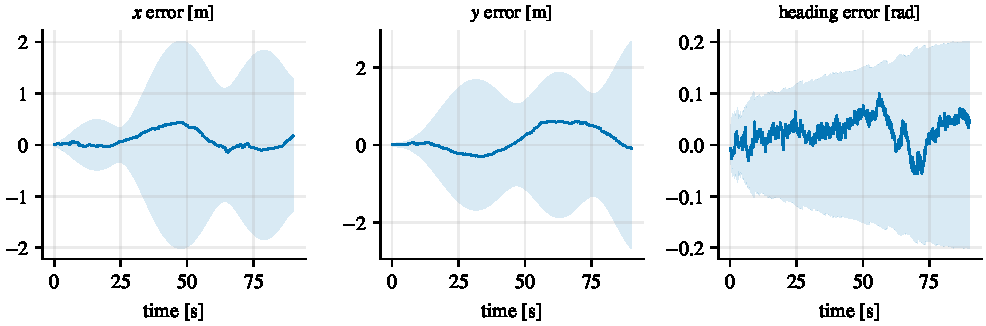
\includegraphics[width=\linewidth]{fig_planar_err.pdf}
\caption{Estimation errors of one run with the filter's $\pm3\sigma$ envelopes (shaded). The position envelopes oscillate because most of the position
uncertainty is perpendicular to the direction of travel, which rotates as the robot circles.}
\label{fig:planar-err}
\end{figure}

\begin{figure}[t]
\centering
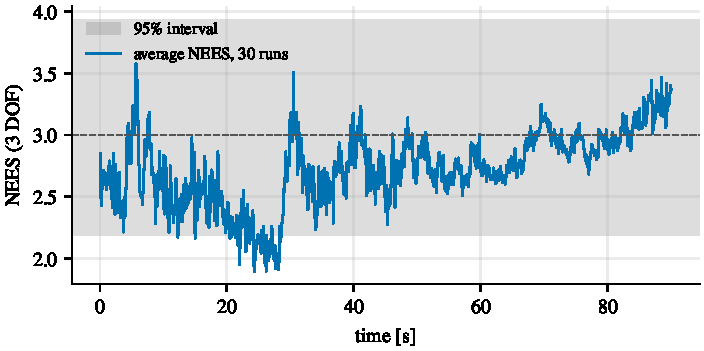
\includegraphics[width=0.8\linewidth]{fig_planar_nees.pdf}
\caption{Average NEES of the robot pose over 30 runs, with the 95\% acceptance interval of \cref{eq:anees-bounds}.}
\label{fig:planar-nees}
\end{figure}

The results (\cref{fig:planar-traj,fig:planar-err,fig:planar-nees}) illustrate four points.
\begin{enumerate}
  \item \textbf{The camera helps, mostly through the heading.} Odometry alone accumulates a heading error with standard deviation
        $\sigma_\omega\sqrt{t} = \SI{0.19}{rad}$ after \SI{90}{s}. The MSCKF ends at about \SI{0.07}{rad}: the camera measures the relative rotation between clones far
        better than the gyro-like turn rate, and because heading errors turn into cross-track position errors, the position error drops by a
        factor of 2.5.
  \item \textbf{The error still grows.} Even with the camera, the heading and position uncertainties grow without bound (\cref{fig:planar-err}).
        This is not a failure: global position and heading are unobservable (\cref{sec:planar-unobservable}), and an odometry filter without loop
        closures can only slow their drift, never stop it. The along-track error is set by the odometry speed noise alone, since a monocular camera
        cannot measure scale (the worked example above).
  \item \textbf{The filter is consistent.} The errors stay inside their $3\sigma$ envelopes, and the average NEES stays inside its acceptance
        interval, apart from mildly conservative dips below it between about 12 and \SI{28}{s}. The gate rejected 5.2\% of the features, close to the 5\% that a $\chi^2_{0.95}$ gate should reject when the filter is
        consistent and every feature is a good one; a much larger rate would signal an overconfident filter or bad data.
  \item \textbf{But the NEES creeps upward.} In the second half of the run its 15-second averages rise steadily, from 2.75 to 2.86 to 3.05, with peaks near 3.5. It is still inside the
        interval, but the trend is systematic: the filter is beginning to believe it knows the heading better than it does. The mechanism, and its cure, are the subject of \cref{ch:observability}.
\end{enumerate}

% ------------------------------------------------------------------------------
\section{The unobservable directions}
\label{sec:planar-unobservable}
\index{unobservable directions!planar}

Suppose we rotate the entire world, the trajectory and every feature, about the origin by a small angle, or translate it. Odometry measures
speed and turn rate in the body frame and does not notice. The camera measures bearings relative to the robot and does not notice either. No
sensor can therefore distinguish the true world from the rotated or translated one: these three directions are \emph{unobservable}
(\cref{sec:observability-linear}), and the filter should never gain information along them.

In error-state coordinates the three directions are the columns of
\begin{equation}
  N = \begin{bmatrix} N_t & N_r \end{bmatrix}, \qquad
  N_t = \begin{bmatrix} I_2 \\ 0 \\ I_2 \\ 0 \\ \vdots \end{bmatrix}, \qquad
  N_r = \begin{bmatrix} \Omega\hat p \\ 1 \\ \Omega\hat p_1 \\ 1 \\ \vdots \end{bmatrix},
  \label{eq:planar-nullspace}
\end{equation}
with one block pair for the robot and one for each clone. $N_t$ shifts every position by the same vector. $N_r$ is the derivative of a rotation
about the origin: a point $p$ moves by $\delta\,\Omega p$, and every heading increases by $\delta$.

\begin{proposition}[The planar nullspace]
\label{prop:planar-nullspace}
If all Jacobians are evaluated at one common set of estimates, then:
\begin{enumerate}
  \item every feature Jacobian satisfies $H_{x,j}N_t + H_{f,j} = 0$ and $H_{x,j}N_r + H_{f,j}\,\Omega\hat p_f = 0$, and therefore the projected Jacobian
        satisfies $H_{o,j}N = 0$;
  \item the exact transition \eqref{eq:planar-phi} maps the nullspace at step $k$ to the nullspace at step $k+1$, $\Phi_kN(\hat x_k) = N(\hat x_{k+1})$;
  \item cloning maps $N$ to the nullspace of the augmented state, $JN = N_{\text{aug}}$.
\end{enumerate}
\end{proposition}
\begin{proof}
(1) Row $i$, translation: $-J_\pi R_i\T + J_\pi R_i\T = 0$. Rotation: using $R_i\T\Omega = \Omega R_i\T$ (\cref{lem:omega}(3)),
\begin{equation*}
  -J_\pi R_i\T\Omega\hat p_i - J_\pi\Omega\hat p_{b,i} + J_\pi R_i\T\Omega\hat p_f = J_\pi\big(\Omega R_i\T(\hat p_f - \hat p_i) - \Omega\hat p_{b,i}\big) = J_\pi(\Omega\hat p_{b,i} - \Omega\hat p_{b,i}) = 0 .
\end{equation*}
Multiplying by $A_j\T$ and using $A_j\T H_{f,j} = 0$ gives $A_j\T H_{x,j}N = 0$.
(2) On the robot block, $\Phi_k(I_2, 0) = (I_2, 0)$, and $\Phi_k(\Omega\hat p_k, 1) = (\Omega\hat p_k + \Omega(\hat p_{k+1} - \hat p_k), 1) = (\Omega\hat p_{k+1}, 1)$; clone blocks are untouched.
(3) The new clone copies the robot's rows of $N$, which are exactly the rows a clone at $\hat p$ should have.
\end{proof}

In words: the linearized filter has the same three unobservable directions as the real system, \emph{as long as every Jacobian uses the same
estimate of each quantity}. A real filter cannot honour this condition. The transition $\Phi_k$ uses $\hat p_{k+1} - \hat p_k$ computed from the
estimate before the update at step $k+1$, while the next transition starts from the corrected estimate; and a clone is linearized at its
current, corrected estimate, not at the value it had when it was created. The identities of \cref{prop:planar-nullspace} then hold only
approximately, the linearized system has an observable heading that the real system does not, and the filter slowly gains spurious heading
information. That is the upward creep in \cref{fig:planar-nees}. \Cref{ch:observability} analyses it in the planar EKF-SLAM setting, where it is most
visible, and shows how First-Estimates Jacobians restore the nullspace.

% ------------------------------------------------------------------------------
\section{From the plane to three dimensions}
\label{sec:planar-to-3d}

\Cref{tab:planar-to-3d} lists every difference between the planar filter and the project's filter. None of them changes the structure of
\cref{alg:planar-msckf}; each changes a formula inside it.

\begin{table}[t]
\centering
\small
\caption{The planar MSCKF and its three-dimensional counterpart.}
\label{tab:planar-to-3d}
\begin{tabularx}{\linewidth}{@{}>{\raggedright\arraybackslash}p{0.2\linewidth}>{\raggedright\arraybackslash}X>{\raggedright\arraybackslash}X@{}}
\toprule
& Plane & Project (AGENTS.md) \\
\midrule
Attitude & heading $\psi$, $R(\psi) = \exp(\psi\Omega)$ & $q_{wb}$, $R_{wb}$, $\Exp$ (\cref{ch:lie}) \\
Error and retraction & $\delta\psi = \psi - \hat\psi$; local and global coincide & local (right) perturbation $q = \hat q\otimes\Exp_q(\delta\theta)$ (C4) \\
Skew operator & $\Omega$, commutes with every $R(\psi)$ & $\sx{\cdot}$; $R\sx{v}R\T = \sx{Rv}$, no commutation \\
Jacobian of $R\T a$ w.r.t.\ the rotation error & $-\Omega R\T a$ & the inverse-action row of \cref{tab:jacobians} \\
Motion sensor & odometry $(v, \omega)$, no biases & IMU $(a_m, \omega_m)$ with gravity and biases (C6) \\
State & $(p, \psi)$ + clones, $3 + 3N$ & $(p, v, q, b_a, b_g)$ + clones, $15 + 6N$ (C3) \\
Camera & 1D bearing $z = y/x$ & 2D normalized $(x/z, y/z)$, through $T_{bc}$ (C6) \\
Constraints per feature & $M - 2$ & $2M - 3$ \\
Reset Jacobian & $1$ & $I - \tfrac12\sx{\delta\hat\theta}$ per attitude (F4) \\
Unobservable directions & 2 translations + heading & 3 translations + yaw (roll and pitch are observable through gravity) \\
\bottomrule
\end{tabularx}
\end{table}

\begin{takeaways}
\begin{itemize}
  \item In the plane every MSCKF Jacobian takes a line: $\partial z/\partial\delta\psi_i = -(1 + z^2)$, $\partial z/\partial\delta p_i = -J_\pi R_i\T$, $H_f = J_\pi R_i\T$.
  \item A camera measures rotation independently of depth, and translation only through parallax ($1/x$).
  \item A feature seen $M$ times gives $M - 2$ constraints in the plane ($2M - 3$ in space); for three views the constraint is a second difference
        that measures the ratio of baselines and the relative headings, but not scale, global position or global heading.
  \item The planar filter is consistent and reduces the dead-reckoning error by a factor of about 2.5, yet its NEES creeps upward: the first sign
        of the spurious heading information studied in \cref{ch:observability}.
  \item The step to three dimensions changes formulas, not structure: non-commuting rotations, the local perturbation, gravity, biases and the reset Jacobian.
\end{itemize}
\end{takeaways}

\begin{exercises}
  \item Verify \cref{prop:planar-H} by finite differences at a random clone pose and feature. Then explain $\partial z/\partial\delta\psi = -(1 + z^2)$ using
        only the bearing angle $\beta = \arctan z$.
  \item Show that $I + F_c\Dt$ and the exact $\Phi_k$ of \eqref{eq:planar-phi} differ by $O(\Dt^2)$, and identify the term.
  \item Add a turn-rate bias $b_\omega$ ($\omega_m = \omega + b_\omega + n_\omega$, $\dot b_\omega = n_b$) to the planar state. Derive the new column of $F_c$ and the new
        row of $G_c$, and show that the bias is observable once the camera sees features. Compare with the gyroscope-bias block of the
        three-dimensional filter.
  \item Repeat the worked example with unequal baselines, $\hat p_3 = (0, 2)$. Find $a$, and show that the projected residual measures the
        ratio of the two baselines.
  \item In the worked example, show that moving the \emph{middle} clone along the viewing direction $x_w$ is invisible to $H_o$, while moving the
        \emph{first} clone along $x_w$ is visible. Interpret the difference in terms of the bearing each clone has to the feature.
  \item Why does a 1D camera need three views of a feature to say anything about the poses, while a 2D camera needs only two? Relate the answer
        to the dimensions of $H_f$.
  \item Run \code{scripts/planar\_sims.py} with window sizes $N_{\max} = 3, 5, 10, 20$ and plot the final RMS position error. Explain the trend, and what
        limits the benefit of a longer window.
  \item Prove part (1) of \cref{prop:planar-nullspace} without using the closed-form Jacobians: argue directly that a measurement function that depends only
        on $R(\psi_i)\T(p_f - p_i)$ cannot change under a common rotation or translation of all positions.
  \item Replace the bearing camera by a range-and-bearing sensor. How many constraints does a feature seen $M$ times give? Which of the unobservable
        directions of \eqref{eq:planar-nullspace} become observable, if any?
\end{exercises}
% Solutions to the exercises of Chapter 27.
\begin{solutions}
  \item At a random clone pose and a feature with $\hat z = 0.3$, central differences with $\varepsilon = 10^{-6}$ agree with \eqref{eq:planar-H} to $10^{-10}$ in all five entries. For the
        heading entry, $\beta = \arctan z$ is the angle between the body axis $x_b$ and the ray to the feature. Turning the robot left by $\delta\psi$ turns the body axis
        toward the ray, so every bearing \emph{decreases} by exactly $\delta\psi$, whatever the depth: $\delta\beta = -\delta\psi$. Since $z = \tan\beta$,
        \[
          \frac{\partial z}{\partial\delta\psi} = \frac{\dd z}{\dd\beta}\,\frac{\partial\beta}{\partial\delta\psi} = \frac{1}{\cos^2\beta}\,(-1) = -(1 + \tan^2\beta) = -(1 + z^2).
        \]
        The factor $1 + z^2$ only converts angle to normalized coordinate: at the edge of the $\pm50^\circ$ field of view it is $2.4$, while in angle every point moves
        by the same $\delta\psi$.

  \item The top-right block of $I + F_c\Dt$ is $\Omega R(\hat\psi_k)e_1v_m\Dt$, while that of $\Phi_k$ is $\Omega(\hat p_{k+1} - \hat p_k) = \Omega R(\hat\psi_k + \tfrac12\omega_m\Dt)e_1v_m\Dt$. With
        $R(\hat\psi_k + \tfrac12\omega_m\Dt) = R(\hat\psi_k)(I + \tfrac12\omega_m\Dt\,\Omega) + O(\Dt^2)$ and $\Omega^2 = -I$,
        \[
          \Phi_k - (I + F_c\Dt) = \begin{bmatrix} 0 & -\tfrac12v_m\omega_m\Dt^2\,R(\hat\psi_k)e_1 \\ 0 & 0\end{bmatrix} + O(\Dt^3).
        \]
        The term is $\tfrac12\Dt^2\,\Omega\ddot{\hat p}$: the nominal path turns during the step, so its displacement is not $\dot{\hat p}_k\Dt$. Note that $F_c^2 = 0$, so for a
        \emph{constant} $F_c$ the matrix exponential would add nothing. The whole difference comes from $F_c$ changing during the step: $I + F_c\Dt$ is the rectangle rule for
        $I + \int F_c\,\dd t$. For the simulation ($v = 1$~m/s, $\omega = 0.1$~rad/s, $\Dt = 0.01$~s) it is $5\times10^{-6}$ per step, relative size $\tfrac12\omega\Dt = 5\times10^{-4}$. It is small,
        but it means the approximate transitions no longer telescope exactly into $\Omega(\hat p_k - \hat p_0)$ (\cref{ch:observability}).

  \item With $\omega = \omega_m - b_\omega - n_\omega$ and the nominal $\dot{\hat\psi} = \omega_m - \hat b_\omega$, $\dot{\delta\psi} = -\delta b_\omega - n_\omega$ and $\dot{\delta b}_\omega = n_b$; the position row is unchanged. For
        $\delta x_R = (\delta p, \delta\psi, \delta b_\omega)$ and $n = (n_v, n_\omega, n_b)$,
        \[
          F_c = \begin{bmatrix} 0_{2\times2} & \Omega R(\hat\psi)e_1v_m & 0_{2\times1} \\ 0 & 0 & -1 \\ 0 & 0 & 0 \end{bmatrix}, \qquad
          G_c = \begin{bmatrix} -R(\hat\psi)e_1 & 0 & 0 \\ 0 & -1 & 0 \\ 0 & 0 & 1 \end{bmatrix},
        \]
        with $Q_c = \diag(\sigma_v^2, \sigma_\omega^2, \sigma_b^2)$: the new column of $F_c$ is $(0, 0, -1, 0)\T$ and the new row of $G_c$ is $(0, 0, 1)$. The camera measures relative headings of
        the clones directly: the heading column $-(1 + z^2)$ does not depend on depth, and turning a single clone is visible. A bias error makes the heading error grow
        linearly across the window, $\delta\psi(t) = \delta\psi_0 - t\,\delta b_\omega$. The unobservable directions cannot produce such a ramp: a global rotation adds the same constant to every
        heading, and translations and scale leave headings unchanged. So the ramp changes the projected residuals, and the bias is observable. Numerically: on
        the simulated circle with ten clones and six landmarks, the observability matrix of $(\delta p, \delta\psi, \delta b_\omega)$ at the first clone time has rank one. Its
        three-dimensional nullspace (the two translations and the rotation) has bias components of $10^{-14}$.
        \ifsolutions
        In three dimensions the attitude row is $\dot{\delta\theta} = -\sx{\hat\omega}\delta\theta - \delta b_g - n_g$ and the bias row $\dot{\delta b}_g = n_{b_g}$. The $-I$ in the gyro-bias columns is the exact
        counterpart of the $-1$ here. The extra term $-\sx{\hat\omega}\delta\theta$ has no planar analog, because a planar heading error does not rotate with the body. For the same
        reason as here, all three gyroscope-bias components are observable once the camera measures relative attitudes: even the bias about the vertical,
        although the global yaw is not.
        \else
        In three dimensions the same mechanism makes all three gyroscope-bias components observable once the camera measures relative attitudes: even the bias
        about the vertical, although the global yaw is not. (The corresponding block of $F_c$ is part of the derivation exercises of \cref{ch:errordyn}.)
        \fi

  \item The body-frame points are $(4, 1)$, $(4, 0)$, $(4, -2)$, so $\hat z = (\tfrac14, 0, -\tfrac12)$ and
        \[
          H_f = \begin{bmatrix} -\tfrac1{16} & \tfrac14 \\ 0 & \tfrac14 \\ \tfrac18 & \tfrac14 \end{bmatrix}, \qquad
          h_1\times h_2 = \tfrac1{64}(-2, 3, -1), \qquad a = \tfrac1{\sqrt{14}}(2, -3, 1),
        \]
        so $r_o = (2r_1 - 3r_2 + r_3)/\sqrt{14}$. For sideways motion at a fixed heading, $z_i = (y_f - y_i)/x_f$ is a linear function of the camera position $y_i = (-1, 0, 2)$, and
        the weights annihilate exactly the constants and the linear functions: $\sum_ia_i = 0$ and $\sum_ia_iy_i = 0$. For baselines $b_1 = y_2 - y_1$ and $b_2 = y_3 - y_2$, the weights are
        $(b_2, -(b_1 + b_2), b_1)$, and $r_o = 0$ exactly when
        \[
          \frac{z_1 - z_2}{z_2 - z_3} = \frac{b_1}{b_2} .
        \]
        The depth $x_f$ cancels in the ratio of image displacements, so the residual compares the observed ratio with the estimated ratio of the baselines, and
        nothing else. If the middle clone were really at $y = 0.1$, the observed ratio would be $1.1/1.9 = 0.58$ instead of $\tfrac12$, and $r_o = -0.020$. The projected Jacobian
        is $H_o = \tfrac1{\sqrt{14}}\big[(\tfrac18, -\tfrac12, -\tfrac{17}8)\ \ (0, \tfrac34, 3)\ \ (-\tfrac18, -\tfrac14, -\tfrac54)\big]$; translation, rotation and scale of the configuration give zero, as before.

  \item With $a = (1, -2, 1)/\sqrt6$, the $\delta p_x$ entries of $H_o$ are $\tfrac{1}{16\sqrt6}$, $0$ and $-\tfrac{1}{16\sqrt6}$. Moving the middle clone along $x_w$ is invisible; moving the first clone
        along $x_w$ is visible, though weakly. The middle clone looks straight at the feature ($\hat z_2 = 0$), so $x_w$ is its own viewing ray, the nullspace of its projection
        Jacobian: moving along the ray changes the depth, which one view cannot see, and leaves the bearing unchanged. The first clone sees the feature at
        $\hat z_1 = \tfrac14$ ($14^\circ$). Moving it along $x_w$ changes that bearing by $\tfrac{1}{16}$ per meter, and the feature cannot absorb the change without disturbing the other two bearings. In
        general, moving a clone along its ray to a feature is invisible in that feature's residual. Other directions are visible, with a sensitivity
        proportional to the sine of the angle between motion and ray, divided by the depth.

  \item Each observation gives as many numbers as the image has dimensions, and the feature has as many unknowns as the space. A 1D camera in the plane: $H_{f,j}$ is
        $M\times2$ of rank 2, leaving $M - 2$ constraints, so $M = 2$ gives none. Two rays in a plane always intersect (unless parallel), so any two bearings are consistent with some
        feature. A 2D camera in space: $H_{f,j}$ is $2M\times3$ of rank 3, leaving $2M - 3$, so $M = 2$ gives one. Two rays in space are generically skew, and requiring them to intersect,
        i.e.\ to be coplanar with the baseline, is the epipolar constraint (Exercise~26.3).

  \item Final RMS errors after 90~s over 30 runs (dead reckoning: $2.80$~m):
        \begin{center}\small
        \begin{tabular}{@{}l c c c c@{}}
        \toprule
        $N_{\max}$ (window length) & 3 (0.3~s) & 5 (0.5~s) & 10 (1~s) & 20 (2~s) \\
        \midrule
        position & 2.23~m & 2.13~m & 0.85~m & 0.33~m \\
        heading & 0.19~rad & 0.17~rad & 0.069~rad & 0.025~rad \\
        average NEES (last 9~s, 3 DOF) & 2.65 & 2.97 & 3.14 & 3.20 \\
        \bottomrule
        \end{tabular}
        \end{center}
        The position error follows the heading error, which turns into cross-track error. The key quantity is how well one window determines the heading
        change across it, a heading ramp, which the camera sees only through parallax. With the scenario's landmarks, a single window determines it with a
        standard deviation of $0.05$, $0.022$, $0.008$ and $0.003$~rad for $N_{\max} = 3$, 5, 10, 20. Odometry alone has $\sigma_\omega\sqrt T = 0.009$, $0.013$, $0.019$ and $0.028$~rad over the same spans.
        Short windows are worse than odometry at exactly the quantity that drives the drift; the camera wins only for windows longer than about half a second,
        which is where the error drops. The benefit then levels off: $0.18$~m at $N_{\max} = 40$ and $0.17$~m at 80. Several things limit it:
        \begin{itemize}
          \item once the window pins the heading change far better than odometry, the remaining error is the unobservable drift of global heading and
                position, which no window removes;
          \item tracks end (here a landmark stays in view for a median of 6.8~s), so a longer window cannot lengthen them;
          \item the cost grows as $n^3$ with $n = 3 + 3N_{\max}$;
          \item old clones are never relinearized;
          \item the NEES creeps upward ($3.24$ at $N_{\max} = 80$), as more constraints feed more spurious heading information (\cref{ch:observability}).
        \end{itemize}

  \item Let $h(x, p_f) = \pi\big(R(\psi_i)\T(p_f - p_i)\big)$, or any function of $R(\psi_i)\T(p_f - p_i)$. Translating everything by $t$ ($p_i \to p_i + t$, $p_f \to p_f + t$) leaves $p_f - p_i$ unchanged.
        Rotating everything about the origin by $\delta$ ($p_i \to R(\delta)p_i$, $\psi_i \to \psi_i + \delta$, $p_f \to R(\delta)p_f$) gives
        $R(\psi_i + \delta)\T R(\delta)(p_f - p_i) = R(\psi_i)\T R(\delta)\T R(\delta)(p_f - p_i) = R(\psi_i)\T(p_f - p_i)$. So $h$ is constant along both families, identically in $t$ and $\delta$.
        Differentiating at $t = 0$ and $\delta = 0$, at the common linearization point $(\hat x, \hat p_f)$: the state moves along $N_t$ and the feature by $I$, or the state along $N_r$ and the
        feature by $\Omega\hat p_f$. Hence
        \[
          H_{x,j}N_t + H_{f,j} = 0, \qquad H_{x,j}N_r + H_{f,j}\,\Omega\hat p_f = 0,
        \]
        and multiplying by $A_j\T$ gives $H_{o,j}N = 0$. Nothing about $\pi$ was used. The proof also shows why the hypothesis matters: the identities come from differentiating one
        function at one point, so they hold only if every block of $H_{x,j}$ and $H_{f,j}$ is evaluated at the same estimates.

  \item Each observation $(\|d_i\|, \atantwo(d_y, d_x))$ now gives two numbers for two unknowns of the feature, so a feature seen $M$ times gives $2M - 2$ constraints. A single
        observation determines the feature and constrains nothing; two observations already give two constraints. None of the directions of
        \eqref{eq:planar-nullspace} becomes observable: the measurement is still a function of $R(\psi_i)\T(p_f - p_i)$ alone, so the argument of Exercise~8 applies unchanged, and global
        translation and heading remain invisible. What changes is scale. The range measures distances, so the shape \emph{and size} of the trajectory are now
        observable from the camera alone, and the along-track error no longer depends on the odometry speed noise only.
\end{solutions}

